% utf-8 ru, unix eolns
\documentclass[12pt,a4paper,oneside]{extarticle}
    \righthyphenmin=2 %минимально переносится 2 символа %%%
    \sloppy

% Рукопись оформлена в соответствии с правилами оформления 
% электронной версии авторского оригинала, 
% принятыми в Издательстве МГТУ им. Н.Э. Баумана.

\usepackage{geometry} % А4, примерно 28-31 строк(а) на странице 
    \geometry{paper=a4paper}
    \geometry{includehead=false} % Нет верх. колонтитула
    \geometry{includefoot=true}  % Есть номер страницы
    \geometry{bindingoffset=0mm} % Переплет    : 0  мм
    \geometry{top=20mm}          % Поле верхнее: 20 мм
    \geometry{bottom=25mm}       % Поле нижнее : 25 мм 
    \geometry{left=25mm}         % Поле левое  : 25 мм
    \geometry{right=25mm}        % Поле правое : 25 мм
    \geometry{headsep=10mm}  % От края до верх. колонтитула: 10 мм
    \geometry{footskip=20mm} % От края до нижн. колонтитула: 20 мм 

\usepackage{cmap}
\usepackage[T2A]{fontenc} 
\usepackage[utf8x]{inputenc}
\usepackage[english,russian]{babel}
\usepackage{misccorr}

\usepackage{amsmath}
\usepackage{amsfonts}
\usepackage{amssymb}

%\usepackage{cm-super} %человеческий рендер русских шрифтов

\setlength{\parindent}{1.25cm}  % Абзацный отступ: 1,25 см
\usepackage{indentfirst}        % 1-й абзац имеет отступ

\usepackage{setspace}   

\onehalfspacing % Полуторный интервал между строками

\makeatletter
\renewcommand{\@oddfoot }{\hfil\thepage\hfil} % Номер стр.
\renewcommand{\@evenfoot}{\hfil\thepage\hfil} % Номер стр.
\renewcommand{\@oddhead }{} % Нет верх. колонтитула
\renewcommand{\@evenhead}{} % Нет верх. колонтитула
\makeatother

\usepackage{fancyvrb}

\usepackage[nounderscore]{syntax} %для поддержки рбнф
%\setlength{\grammarindent}{12em} %устанавливает нужный отступ перед ::=
\setlength{\grammarparsep}{6pt plus 1pt minus 1pt}  %сокращает расстояние между правилами

\usepackage[pdftex]{graphicx}  % поддержка картинок для пдф
\graphicspath{ {./pictures/} }
\usepackage{rotating}
%\DeclareGraphicsExtensions{.jpg,.png}

\renewcommand{\labelenumi}{\theenumi.} %меняет вид нумерованного списка

\usepackage{perpage} %нумерация сносок 
\MakePerPage{footnote}

\usepackage[all]{xy} %поддержка графов

\usepackage{listings} %листинги
\renewcommand{\lstlistingname}{Листинг}
\lstset{
  basicstyle=\small,
  breaklines=true
  }

\usepackage{url}


\usepackage{tikz} %для рисования графиков
\usepackage{pgfplots}


\usepackage{ccaption}%изменяет подпись к рисунку
\makeatletter 
\renewcommand{\fnum@figure}[1]{Рисунок~\thefigure~---~\sffamily}
\makeatother



\begin{document}
\pgfplotsset{compat=1.8}

\thispagestyle{empty}
\newpage
{
\centering


\textbf{
МОСКОВСКИЙ ГОСУДАРСТВЕННЫЙ ТЕХНИЧЕСКИЙ УНИВЕРСИТЕТ ИМЕНИ Н. Э. БАУМАНА \\
Факультет информатики и систем управления \\
Кафедра теоретической информатики и компьютерных технологий}
\bigskip
\bigskip
\bigskip
\bigskip
\bigskip
\bigskip
\bigskip

\vfill

Курсовой проект \\
по курсу <<Конструирование компиляторов>>

\bigskip

{\large <<Препроцессор синаксического сахара для языка Scheme>>}
\bigskip

\vfill



\hfill\parbox{4cm} {
Выполнил:\\
студент ИУ9-101 \hfill \\
Выборнов А. И.\hfill \medskip\\
Руководитель:\\
Дубанов А. В.\hfill
}


\vspace{\fill}

Москва \number\year
\clearpage
}


\tableofcontents

\clearpage

\begin{itemize}
    \item про замыкания в определении функций и анонимных функциях
    \item куда вписать про стандартные функции

\item косяк с видимостью символов внутри функции (всё же def надо заменить на let)

\end{itemize}

\clearpage

\section*{Введение}
\addcontentsline{toc}{section}{Введение}
    Lisp~---~это семейство динамических функциональных языков программирования.
    Первая версия языка Lisp была создана в 1958 году в ходе работ по созданию искусственного интеллекта.
    К настоящему времени сфера применения Lisp значительно увеличилась, а Lisp представляет собой целое семейство языков: Сommon Lisp, Scheme, Racket и другие. 

    В рамках работы рассматривается язык Scheme.
    Этот язык был разработан специально для учебных целей, благодаря чему включает в себя очень ограниченный, но весьма гибкий набор примитивов.
    Scheme удобен для написания скриптов и расширений~(имеется специально для этого предназначенная реализация~---~GNU Guile).

    Форматирование кода на Scheme, отслеживание парных открывающих и закрывающих скобок и некоторые другие синтаксические особенности требуют применения не слишком распространенных и привычных приложений таких как специализированная среда разработки, к примеру~---~Racket или текстовый редактор со специальными расширениями, наиболее часто используется Emacs. 

    К числу недостатков можно также отнести: обилие скобок, затрудняющее чтение программы, отсутствие возможности записи выражений в привычном инфиксном формате.

    В последнее время отмечается значительный рост интереса к практическому применению функционального программирования, а таже удобству чтения и написания кода.
    Это привело к созданию большого числа языков программирования, в той или иной степени использующих синтаксис и семантику языка ML~(Meta Language).
    В реализациях этих языков основной упор сделан на типобезопасность.
    Языки являются компилируемыми, со строгой статической типизацией.
    Интроспекция в этих языках затруднена.

    Целью данной работы является разработка и реализация функционального динамического языка на основе Scheme, который имеет более дружелюбный синтаксис.

    На разработку входного языка сильное влияние оказал Haskell~\cite{haskell}~---~представитель семейства ML подобных языков, который много унаследовал от Scheme: управляющие конструкции, связывание имён со значениями и т.д.
    В качестве целевого языка используется язык Scheme, удолетворяющий стандарту r5rs~\cite{r5rs}.

    Компилятор входного языка в целевой реализован как препроцессор к языку Scheme.

    Входной язык и компилятор получили название lactose~(лактоза~---~молочный сахар).
    Названия языка это отсылка как к синтаксическому сахару, так и первоначальному обучению программированию.
\clearpage

\section{Теоретическая часть}
    \subsection{Scheme}
        Scheme~---~функциональный язык программирования.
        При разработке Scheme был сделан упор на элегантность и простоту языка.
        В результате, Scheme содержит минимум примитивных конструкций и позволяет выразить всё, что угодно путём надстройки над ними.

        Racket~---~мультипарадигменный язык программирования общего назначения, принадлежащий семейству Lisp/Scheme.
        Одно из предназначений Racket~---~создание, разработка и реализация языков программирования.
        Racket это не просто язык программирования, а целая платформа, которая предоставляет реализацию языка Racket, развитую среду выполнения, различные библиотеки, JIT-компилятор, а также среду разработки DrRacket (ранее известную, как DrScheme) написанную на Racket.

        Racket поддерживает исполнение программ написанных согласно стандарту Scheme r5rs.

        Результатом работы компилятора является файл Racket, содержащий в себе программу на языке Scheme.
    \clearpage

    \subsection{Входной язык \textcolor{red}{ДОПИСАТЬ}}
        Программа на входном языке представляет собой множество определений функций и операторов, которые позволяют импортировать символы из Scheme.
        Если в корне программы определена функция main, то она будет являться точкой входа.

        %переменные
        %видимость??!

        \subsubsection{Токены}
            Токены языка аналогичны токенам языка программирования Scheme.
            Представлены следующие виды токенов: строка, идентификатор, число, логический тип и символ (литеральная константа). Примеры правильных токенов: 

            \begin{itemize}
                \item символ закрывающей скобки~---~\lstinline$#\)$
                \item строка~---~\lstinline$"\"r5rs\" standart\n"$
                \item идентификатор~---~\lstinline$_ident$
                \item логическая истина~---~\lstinline$#t$
                \item десятичное число~---~\lstinline$123$
                \item шестнадцатеричное число~---~\lstinline$#xDEADBEAF$
            \end{itemize}

            В рамках грамматики под нетерминалом $\langle token\rangle$ подразумевают строку, число, логический тип или символ:
            \begin{grammar}
                <token> ::= <BOOLEAN> | <NUMBER> | <CHARACTER> | <STRING>
            \end{grammar}
            Терминал, соответствующий идентификатору~---~$\langle IDENTIFIER \rangle$, рассматривается отдельно.

            Единственным существенным отличием лексической структуры входного языка от Scheme является отсутствие знака перед числом, так как во входном языке знак перед числом определяется с помощью унарного минуса, который, в свою очередь, встроен в интерпретатор и фактически является элементом синтаксиса языка.
            Зависимость от регистра символов определяется настройками интерпретатора Scheme, работающем в связке с нашим компилятором.            

            Документация Sсheme~\cite{r5rs} содержит следующее определение строки в РБНФ:
            \begin{grammar}
                <string> ::= `"' <string element>* `"'

                <string element> ::= any character other than `"' or `\textbackslash' | `\textbackslash "' | `\textbackslash \textbackslash'
            \end{grammar}
            Данное определение содержит ошибку.
            Оно не позволяет определить одиночный слэш.
            Поэтому использовалось определение строки, совпадающее с таковым в реализации стандарта r5rs в рамках языка Racket: 
            \begin{grammar}
                <string> ::= `"' <string element>* `"'

                <string element> ::= любой символ кроме `"' или `\textbackslash' | `\textbackslash "' | `\textbackslash'
            \end{grammar}

        \subsubsection{Выражения}
            Основной структурной единицей языка является выражение.
            В качестве выражения рассматриваются унарные и бинарные инфиксные операции, условный оператор, вызов функции, анонимные функции, списки.
            Входной язык поддерживает инфиксные операции, аналогичные операциям языка Python.
            Порядок вычислений определяется приоритетом операторов, а также может быть задан явно с помощью круглых скобок.

            Выражение задаётся нетерминалом $\langle expression \rangle$. Грамматика выражений в формате РБНФ:
            \begin{grammar}
                <expression> ::=
                      <arithmetic expression> \\
                    | <lambda function> \\
                    | <list expression> \\

                <arithmetic expression> ::=
                      <arithmetic expression> `**' <arithmetic expression> \\
                    | <arithmetic expression> (`*'|`/'|`\%'|`//') <arithmetic expression> \\
                    | <arithmetic expression> (`+'|`-') <arithmetic expression> \\
                    | <arithmetic expression> (`\textless\null\textless' | `\textgreater\null\textgreater') <arithmetic expression> \\
                    | <arithmetic expression> `&' <arithmetic expression> \\
                    | <arithmetic expression> `^' <arithmetic expression> \\
                    | <arithmetic expression> `|' <arithmetic expression> \\
                    | <arithmetic expression> `and' <arithmetic expression> \\
                    | <arithmetic expression> `or' <arithmetic expression> \\
                    | <arithmetic expression> (`\textless' | `\textless=' | `\textgreater' | `\textgreater=') <arithmetic expression> \\
                    | <arithmetic expression> (`==' | `!=') <arithmetic expression> \\
                    | (`+'|`-') <arithmetic expression> \\
                    | (`not'|`~') <arithmetic expression> \\
                    | <if condition> \\
                    | <token> \\
                    | <IDENTIFIER> \\
                    | <function call> \\
                    | <lambda function call> \\
                    | `(' <arithmetic expression> `)'
            \end{grammar}

            Приоритеты заданы в РБНФ следующим образом: если тело правила состоит из нескольких частей, разделённых знаком `|', то чем левее часть, тем у неё выше приоритет.

            Пример выражения: \lstinline$not (x > 2 and x < 5)$.

        \subsubsection{Условия}
            В качестве условного оператора используется традиционный оператор if. В грамматике условный оператор задаётся с помощью нетерминала $\langle if~condition \rangle$. Условный оператор в формате РБНФ:
            \begin{grammar}
                <if condition> ::= `if' <expression> `then' <expression> `else' <expression>
            \end{grammar}
            Условный оператор работает аналогично тернарному оператору: если выражение после `if' истинно, то он возвращает выражение после `then', в противном случае он возвращает выражение после `else'.

            Пример условия: \lstinline$if not (x > 2 and x < 5) then 1 else 0$.

        \subsubsection{Определение функций}
            Определение функции начинается с ключевого слова `def'.
            Функция задаётся идентификатором, соответствующим имени функции, списком идентификаторов, которые соответствуют аргументам функции и телом функции.
            Тело функции состоит из последовательности определений функций и выражений, которые, при вызове функции, последовательно исполняются.
            Функция возвращает результат последнего выражения из тела функции.

            В грамматике определение функции соответствует нетерминалу $\langle function~define \rangle$. Синтаксис определения функции в РБНФ:

            \begin{grammar}
                <function define> ::= `def' <IDENTIFIER> <function arguments> `=' ( <function body> | `{' <function body> `}' )

                <function body> ::= <function_body_token> (`;' <function_body_token>)*

                <function body token> ::= <function define> | <expression>;

                <function arguments> ::= <IDENTIFIER>*
            \end{grammar}

            Пример определения функции \lstinline$abs$ от одного аргумента, которая возвращает модуль числа: \lstinline$def abs a = if a < 0 then -a else a$.
        \subsubsection{Локальные определения функций \textcolor{red}{ДОПИСАТЬ}}
            написать после фикса баги :( 

            доп текст есть на бумажке
            %В отличие от Scheme локальные определения соответствуют let и letrec

            %описать про проблему с распознованием конца функции. Поэтому тело можно внести в {}

        \subsubsection{Анонимные функции}
            Грамматика языка поддерживает анонимные функции~($\lambda$-функции). Анонимные функции особый вид функций, которые объявляются в месте использования и не получают уникального идентификатора для доступа к ним. Анонимные функции можно либо вызвать напрямую при создании, либо присвоить ссылку на неё в переменную~(в контексте входного языка в функцию), для косвенного вызова в дальнейшем.

            Анонимной функции соответствует нетерминал $\langle lambda~function \rangle$. Cинтаксис анонимной функции в РБНФ:
            \begin{grammar}
                <lambda function> ::= `\\' <function arguments> `->' <function body>
            \end{grammar}

            Пример анонимной функции от двух аргументов, которая находит сумму квадратов двух чисел: \lstinline$\x y-> x*x + y*y$.

        \subsubsection{Вызов функций}
            Вызов функции представляет собой имя функции и список выражений, соответствующих аргументам функции.
            При вызове анонимной функции имя заменяется на определение анонимной функции, заключённое в круглые скобки.

            В грамматике вызовы функций задаются нетерминалами $\langle function~call \rangle$ и $\langle lambda~function~call \rangle$, для обычных и анонимных функций соответственно. Синтаксис вызовов функций в РБНФ:

            \begin{grammar}
                <function call> ::= <IDENTIFIER> <expression>*

                <lambda function call> ::= `(' <lambda function> `)' <expression>*
            \end{grammar}

            Пример определения рекурсивной функции \lstinline$fact$ от одного аргумента, которая находит факториал числа: \lstinline$def fact n = if n == 0 then 1 else n*(fact n-1)$. Пример содержит вызов функции \lstinline$fact$.

            Пример вызова анонимной функции от одного аргумента, который также является анонимной функцией: \lstinline$(\f -> f 3) \x->x**2$.

        \subsubsection{Cписки}
            Во входном языке список это набор выражений, который обрамляется квадратными скобками.
            Список напрямую отображается в список языка Scheme.
            Для работы со списками определён набор функций~(в круглых скобках указывает аналог из языка Scheme, при наличии):
            \begin{itemize}
                \item len~(length)~---~принимает на вход список и возвращает длину списка.
                \item concat~(append)~---~принимает на вход произвольное количество списков и возвращает список, представляющий собой конкатенацию переданных списков.
                \item ref~(list-ref)~---~принимает на вход список~(lst) и число~(pos), возврашает элемент списка lst под номером pos~(нумерация элементов списка начинается, как и в Scheme с нуля).
                \item head~---~принимает на вход список~(lst) и число~(pos), возвращает список, состоящий из элементов lst с номером меньшим pos в том же порядке.
                \item tail~(list-tail)~---~принимает на вход список~(lst) и число~(pos), возвращает список, состоящий из элементов lst с номером большим либо равным pos в том же порядке.
            \end{itemize}

            В грамматике список задаётся нетерминалом $\langle list~expression \rangle$. Cинтаксис списка в РБНФ:
            \begin{grammar}
                <list expression> ::= `[' expression* `]'
            \end{grammar}

            Пример списка, содержащего два числа: \lstinline$[1 2+3]$.

        \subsubsection{Комментарии}
            Комментарии представляют собой часть строки, которая начинается с символа `--' и заканчивается переводом строки.
            Комментарии препроцессором полностью игнорируются.

            Синтаксис нетерминала $\langle comment \rangle$, соответствующего комментарию, в формате РБНФ:

            \begin{grammar}
                <comment> ::= `-\null-' (любой символ кроме `\\n')*;
            \end{grammar}

            Пример комментария: \lstinline$-- commented text\n$
            

        \subsubsection{Импортирование символов из Scheme}
            Входной язык поддерживает импорт символов функций из Scheme.
            Для это необходимо написать произвольный код на Scheme, обрамлённый с помощью двойных фигурных скобок, и, после ключевого слова `export', описать импортированную функцию.

            Под описанием импортированной функции подразумевается идентификатор, задающий имя функции и список аргументов.
            В качестве списка аргументов рекомендуется либо передать единственный аргумент `\_', если функция принимает какие-либо аргументы на вход, либо ничего не передавать в противном случае.

            Импорт символов из Scheme в грамматике описывается нетерминалом $\langle scheme~block \rangle$. Синтаксис импорта символов в формате РБНФ:            
            \begin{grammar}
                <scheme block> ::= <SCHEME BODY> `export' <IDENTIFIER> <function arguments> 

                <SCHEME BODY> ::= `{{' (любой символ кроме `}')* `}}'
            \end{grammar}

            Пример определения функции, печатающей квадрат переданного числа в консоль, на языке Scheme и экспорта символа этой функции в lactose: \lstinline${{(define (print_sqr x) (display (expt x 2)))}} export print_sqr _$.
            Пример импортирования функции \lstinline$car$ из стандартной библиотеки Scheme в lactose: \lstinline${{}} export car _$.
        
\clearpage

\section{Реализация}
    Компиляция входного языка состоит из трёх основных этапов: 
    \begin{enumerate}
        \item Лексический и синтаксический анализ входного языка, получение абстрактного синтаксического дерева.
        \item Семантический анализ, во время которого синтаксическое дерево входного языка преобразуется в абстрактное синтаксическое дерево языка Scheme.
        \item По дереву языка Scheme порождается файл, который является программой на Racket.
    \end{enumerate}

    На первом этапе, с помощью лексера и парсера, созданных генератором парсеров ANTLR~(описан в главе~\ref{subsec:antlr}) выполняется лексический и синтаксический анализ.
    По завершении анализа ANTLR возвращает абстрактное синтаксического дерево, которое преобразуется в внутренний формат препроцессора: каждый узел расширяется с помощью дополнительной информации~---~таблица символов, уникальные идентификаторы узлов и т.д..

    На следующем этапе выполняется семантический анализ, который заключается в рекурсивном обходе абстрактного синтаксического дерева.
    Рекурсивный обход выполняется с помощью рекурсивного спуска~---~каждая вызываемая при обходе функция соответствует одному токену из грамматики входного языка.
    Во время обхода порождается синаксическое дерево языка Sсheme~---~иерархическая структура из списков и строк, а также проверяется видимость символов, а именно, идентификаторов.

    На третьем этапе по иерархической структуре из списков и строк, содержащей абстрактное синтаксическое дерево языка Scheme порождается файл, который является программой на Racket.
    Если функция main определена в теле программы, то в конец файла добавляется её вызов.

    \clearpage

    \subsection{Особенности реализации}
        \subsubsection{Обработка ошибок}
            \label{subsubsec:error}
            Все ошибки условно делятся на две группы~---~синтаксические и семантические ошибки.

            Синтаксические ошибки~---~это ошибки возникающие в лексическом и синтаксическом анализаторах.
            Эти ошибки порождаются с помощью классов, сгенерированных ANTLR.

            В ANTLR предусмотрен интерфейс для изменения поведения лексера и парсера при возникновении ошибки.
            Этот интерфейс представляет собой работу с наследниками класса ErrorListener.
            ErrorListener определяет поведение лексера или парсера при возникновении синтаксической ошибки.
            Можно добавлять или удалять наследников класса ErrorListener, тем самым модифицируя обработку ошибок.

            В версии ANTLR для Java данный механизм полноценно работает, но в Python версии ANTLR находится только ядро этого механизма и отсутствуют такой важный функционал, как удаление наследников класса ErrorListner.
            То есть можно расширишить уже существующую обработку ошибок, но переопределить её нельзя.
            Из-за описанного недостатка Python версии ANTLR необходимо обращаться к приватной переменной, содержащей наследников класса ErrorListner для переопределения обработки ошибок.

            Семантические ошибки~---~это ошибки возникающий при семантическом разборе. В рамках данной работы рассматривалась только одна семантическая ошибка~---~идентификатор не найден.

            Все ошибки выводятся в момент возникновения в формате: [line,~column]:~message, где line~---~номер строки во входном файле, column~---~номер столбца во входном файле, message~---~сообщение об ошибке.

            Если по завершении лексического и синтаксического анализа произошла хотя бы одна синтаксическая ошибка, то выполнение прерывается. Если синтаксических ошибок не было, то начинает работу семантический анализатор. 

            Если по завершении семантического анализа произошла хотя бы одна семантическая ошибка, то выполнение прерывается. Если семантических ошибок не было, то порождается результирующий файл.

        \subsubsection{Области видимости символов \textcolor{red}{ДОПИСАТЬ}}
            \textcolor{red}{дописать как пофиксятся вложенные функции}

            Для проверки символов на доступность используются таблицы символов.
            Таблица символов для узла дерева синтаксического разбора~---~это отображение идентификаторов символов, видимых в этом узле, в описания соответствующих этим символам сущностей.

            В реализации препроцессора таблицы символов хранятся только в корневом узле, а также в узлах соответствующих определениям функций (как обычных, так и анонимных). Таблицы символов заполняется одновременно с преобразованием абстрактного синтаксического дерева ANTLR в внутренний формат препроцессора. В таблицу символов для узла попадают все функции определённые на нижележащем уровне дерева. Для каждой функции, в узле её определяющем, хранится список аргументов.

            На этапе семантического анализа для каждого идентификатора выполняется подъём по абстрактному синтаксическому дереву. Если на каком-либо уровне находится либо символ из таблицы, либо аргумент из функции совпадающий с идентификатором, то семантический анализ продолжается, иначе считается, что данный идентификатор на найден и печатается сообщение об ошибке.

        \subsubsection{Защитное программирование}
            Зашитное программирование~---~способ написания программ при котором появляющиеся ошибки легко обнаруживаются и идентифицируются программистом.
            При написании компилятора использовался такой метод защитного программирования, как утверждения.

            Утверждение~(assertion)~---~код, используемый во время разработки, с помощью которого программа проверяет правильность своего выполнения. Утверждения используются для прерывания программы на ситуациях, которые никогда не должны были произойти~\cite{mcconnell}.

            Язык Python поддерживает использование утверждений с помощью ключевого слова `assert'. 

            В препроцессоре на стадии семантического анализа используются утверждения. Каждая функция, являющаяся частью рекурсивного спуска проверяет узел синтаксического дерева, передаваемый на вход, на совпадение с ожидаемым типом этого узла.

        \subsubsection{Тестирование}
            Для повышения эффективности разработки применяется модульное тестирование.
            В качестве программного обеспечения для тестирования используется фреймворк unittest.

            Фреймворк unittest входит в стандартную библиотеку Python и служит базовым инструментом для организации модульных тестов.

            В рамках работы выполняется тестирование результатов компиляции входного языка в Scheme.
            Для этого функционал входного языка разделён на небольшие смысловые части: токены, строки, комментарии, условия, вызовы функций и т.д..
            Для каждой части функционала входного языка написан набор тестов, по-возможности, покрывающий все возможные сценарии работы.
    \clearpage

    \subsection{Используемые технологии}
        \subsubsection{ANTLR}
            \label{subsec:antlr}
            ANTLR (ANother Tool for Language Recognition)~---~генератор нисходящих анализаторов для формальных языков.
            ANTLR преобразует контекстно-свободную грамматику в виде РБНФ в программу на C++, Java, C\#, Python, Ruby.
            В препроцессоре используется ANTLR версии 4.
            С помощью него порождается лексический и синтакический анализаторы для языка Python.

            Преимуществами ANTLR являются: использование единой нотации грамматики как для генератора лексического, так и для генератора синаксического анализатора, применение нисходящего анализа, предоставление сообщений об ошибках.

            Главным недостатком ANTLR, в отличие от Flex/Bison, является использование LL-анализатора, заместо более быстрого LALR.
            Cтоит отметить, что в ходе использования выяснились многие проблемы версии ANTLR для Python:
            \begin{itemize}
                \item отсутствие документации~---~разработчики предполагают использование документацию для Java версии ANTLR,
                \item ограниченный функционал~---~многие элементы интерфейса ANTLR, описанные в документации для Java версии ANTLR, не реализованы, это вызвало проблемы при обработке ошибок~(подробнее в главе~\ref{subsubsec:error}),
                \item незадокументированные различия в поведении классов InputStream и FileStream, превращающих в поток символов строку и текстовый файл соответственно,
                \item низкая производительность~(подробнее в главе~\ref{subsubsec:perfomance}).
            \end{itemize}

            ANTLR поставляется в виде библиотеки для языка Python~---~antlr4-python2-runtime, а также java-приложения.
            С помощью java-приложения по описанию грамматики генерируются файлы на языке Python, содержащие лексический и синтаксический анализаторы.
            При наличии установленной библиотеки antlr4-python2-runtime, полученные анализаторы можно использовать в произвольных Python-приложениях.            
        \subsubsection{Graphviz}
            Graphviz (сокращение от англ. Graph Visualization Software)~---~пакет утилит по автоматической визуализации графов, заданных в виде описания на языке DOT.

            Graphviz используется для визуализации абстрактного синтаксического дерева.
            По синтаксическому дереву генерируется файл на языке DOT, который с использованием утилиты dot из пакета graphviz преобразуется в изображение абстрактного синтаксического дерева в формате pdf.
    \clearpage

    \subsection{Установка}
        Установка приложения происходит в два этапа: генерация лексического и синтаксического анализаторов с помощью ANTLR (описано в главе~\ref{subsec:antlr}) и установка препроцессора в виде пакета на языке python.
        
        Для установки препроцессора используется пакет distutils, который входит в стандартную библиотеку Python.
        Пакет distutils обеспечивает сборку и установку дополнительных модулей для языка Python.
        На листинге~\ref{lst:setup} показан скрипт, конфигурирующий distutils.
        В нём устанавливается две точки входа: одна для препроцессора~(lactose), другая для модуля тестирования~(tests), зависимость от пакета antlr4-python2-runtime, а также указывается какую точку входа использовать для тестирования.

        \begin{figure}[h!]  
            \begin{lstlisting}[label={lst:setup},caption={Cкрипт конфигурации для утилиты distutils},captionpos=b]
from setuptools import setup, find_packages

setup(name='lactose',
      packages=find_packages(),
      entry_points = {
        'console_scripts': [
            'lactose = lactose.main:main',
            'tests = tests.tests:main',
        ]
      },
      install_requires=['antlr4-python2-runtime'],
      zip_safe=False,
      test_suite="tests")

            \end{lstlisting}
        \end{figure}

        Для связки двух этапов используется make~---~утилита, автоматизирующая процесс преобразования файлов из одной формы в другую.
        Утилита make использует файл конфигурации: Makefile.
        Ипользуемый Makefile приведён на листинге~\ref{lst:makefile}.
        Данный Makefile позволяет устанавливать пропроцессор в директорию, конфигурируемую с помощью переменной окружение PREFIX, а также очищать временные файлы, которые генерируются при сборке пакета.

        \begin{figure}[h!]  
            \begin{lstlisting}[label={lst:makefile},caption={Cкрипт конфигурации для утилиты make},captionpos=b]
PREFIX ?= /usr/local
BIN_DIR = $(PREFIX)/bin
LIB_DIR = $(PREFIX)/lib/python2.7/site-packages


INSTALL_TARGETS = install-dir install-package clean

install: $(INSTALL_TARGETS)

install-dir:
    install -d $(PREFIX) $(BIN_DIR) $(LIB_DIR)

install-package: install-dir clean
    java -jar ./lib/antlr-4.5-complete.jar -Dlanguage=Python2 \
        ./lactose/grammar/lactose.g4
    PYTHONPATH=$(LIB_DIR) python setup.py test install --prefix=$(PREFIX)
    @echo 'Lactose successfully installed'

clean:
    @find . -name \*.pyc -delete
    @rm -rf build dist lactose.egg-info

            \end{lstlisting}
        \end{figure}

        \noindent Установка препроцессора состоит из следующих шагов:
        \begin{enumerate}
                \item получение свежей версии препроцессора из репозитория,
                \item установка пакета antlr4-python2-runtime,
                \item установка препроцессора с помощью утилиты make,
                \item eсли требуется функционал по выводу синтаксического дерева в pdf файл, то также необходимо установить пакет graphviz.
        \end{enumerate}

        \noindentПример установки препроцессора, использующий утилиты: git, pip и apt:  
        \begin{lstlisting}
    pip install antlr4-python2-runtime
    apt-get install graphviz
    git clone https://github.com/art-vybor/lactose.git
    cd lactose
    make install
        \end{lstlisting}
    \clearpage
    
    \subsection{Интерфейс}
        Препроцессор является приложением, предоставляющим интерфейс командной строки~(в квадратных скобках указаны необязательные параметры):
        \begin{lstlisting}        
    lactose [-h] -i filename [-o filename] [--run]
           [--stack_trace] [--lexems] [--console_tree] [--pdf_tree]
        \end{lstlisting}

        \noindentИнтерфейс командной строки обеспечивает доступ к основным функциям и настройкам:
        \begin{itemize}
                \item печать справки по интерфейсу командной строки~(ключ \lstinline$-h$),
                \item параметризация входного файла~(параметр \lstinline$-i$),
                \item параметризация выходного файла~---~по умолчанию создаёт выходной файл рядом с входным с заменой расширения файла на ``rkt''~(параметр \lstinline$-o$),
                \item немедленное выполнение программы после компиляции~(ключ \lstinline$--run$),
                \item печать стека вызовов при возникновении ошибки~(ключ \lstinline$--stack_trace$),
                \item вывод распознанных лексем~(ключ \lstinline$--stack_trace$),
                \item вывод дерева разбора в консоль~(ключ \lstinline$--console_tree$),
                \item вывод дерева разбора в графическом виде в файл PDF~---~создаёт файл рядом с входным с заменой расширения файла на ``pdf''~(параметр~(ключ \lstinline$--pdf_tree$).
        \end{itemize}

        \noindentПример компиляции файла sample.lc с последующим запуском:
        \begin{lstlisting}        
    lactose -i sample.lc --run
        \end{lstlisting}
\clearpage

\section{Тестирование}
    \subsection{Удобство использования \textcolor{red}{ДОБАВИТЬ ПРИМЕРОВ, ДОПИСАТЬ}}
        Удобство использования достаточно субъективная метрика. ...

        \begin{table}[h!]
            \label{tabular:syntax}
            \centering        
            \begin{tabular}{|l|l|}
                \hline
                \textbf{Входной язык} & \textbf{Scheme}
                \\ \hline
                    \begin{lstlisting}
def abs x = if x < 0 then -x else x
                    \end{lstlisting} &
                    \begin{lstlisting}
(define (abs x) (if (< x 0) -x x))
                    \end{lstlisting}
                \\ \hline
                    \begin{lstlisting}
def fact n = 
    if n == 0 then 1
    else n*(fact n-1)
                    \end{lstlisting} &
                    \begin{lstlisting}
(define (fact n)
    (if (= n 0) 1
        (* n (fact (- n 1)))))
                    \end{lstlisting}
                \\ \hline
                    \begin{lstlisting}
def make_adder n = \x -> x+n
                    \end{lstlisting} &
                    \begin{lstlisting}
(define (make_adder n) 
  (lambda (x) (+ x n)))
                    \end{lstlisting}
                \\ \hline
                % пример на вложенные функции
            \end{tabular}
        \caption{Сравнение входного языка и Scheme}
        \end{table}

В таблице~\ref{tabular:syntax} приведены реализации одних и тех же функций на входном языке и на Scheme. Как видно из таблицы ...

    \clearpage

    \subsection{Производительность}
        \label{subsubsec:perfomance}
        Во время разработки обнаружен факт очень медленной компиляции даже небольших программ.
        Был составлен тест, состоящий из множественного определения функций \lstinline$abs$, вида: \lstinline$def abs{INDEX} x = if x >= 0 then x else -x$, где {INDEX}~---~целое число, уникальное для каждого определения функции.        
        \begin{figure}[h!]        
        \centering
            \begin{tikzpicture}[scale=2]
                \begin{axis}[ ylabel=время компиляции (с), xlabel=количество определённых функций,
                ] \tiny
                    \addplot coordinates {                            
                        (10, 0.154279947281)
                        (20, 0.197158098221)
                        (30, 0.30188703537)
                        (40, 0.3914539814)
                        (50, 0.514985799789)
                        (60, 0.608325004578)
                        (70, 0.713381767273)
                        (80, 0.792292833328)
                        (90, 0.881745100021)
                        (100, 0.976894855499)
                        (110, 1.11551380157)
                        (120, 1.17175197601)
                        (130, 1.27003216743)
                        (140, 1.41063594818)
                        (150, 1.47410702705)
                        (160, 1.59055113792)
                        (170, 1.66601586342)
                        (180, 1.83970785141)
                        (190, 1.85405898094)
                        (200, 2.04520893097)
                        (210, 2.04659700394)
                        (220, 2.24038600922)
                        (230, 2.42818903923)
                        (240, 2.49178504944)
                        (250, 2.89057707787)
                        (260, 2.79826784134)
                        (270, 3.29559087753)
                        (280, 3.14558386803)
                        (290, 3.18815994263)
                    };
                \end{axis}
            \end{tikzpicture}
        \caption{Результаты тестирования производительности}
        \label{pic:test}
        \end{figure}
        На рисунке~\ref{pic:test} показан график зависимости времени компиляции от количества определённых функций \lstinline$abs$ в теле программы. Как видно из рисунка время компиляции программы линейно зависит от количества определений. При этом абсолютное значение времени достаточно велико~---~для программы из 100 определений порядка 1 секунды.

        Для определения узкого места в программе, воспользуемся профилировщиком cProfile и визулизатором gprof2dot.
        Профилировщик находит время выполнения каждой функции программы, а визуализатор строит дерево выполнения программы в формате dot.
        Для каждой функции создаётся узел дерева, содержащий информацию об имени функции, проценте времени, затраченного на выполнение функции, относительно времени работы всей программы и количестве вызовов функции.
        Получившееся дерево можно визуализировать с помощью утилиты graphviz.

        \begin{figure}[h!]
            \center
            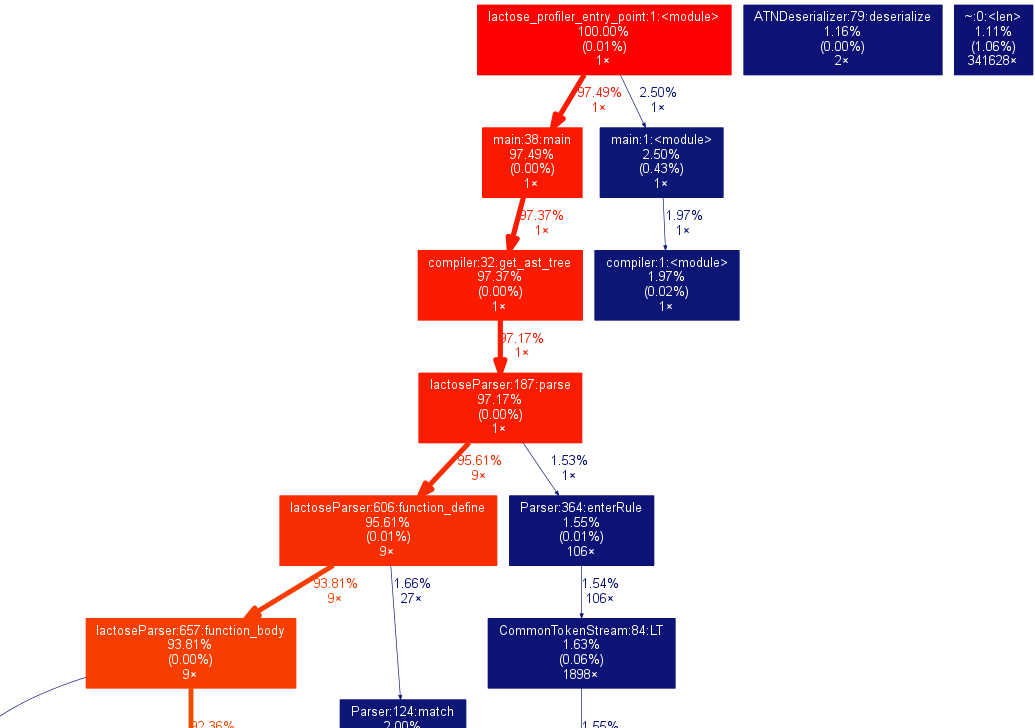
\includegraphics[scale=0.3]{lactose_stats.png}
            \caption{Результат работы профилировщика}
            \label{pic:stats}
        \end{figure}

        Часть получившегося дерева, приведена на рисунке~\ref{pic:stats}~(использованы настройки gprof2dot, которые отсекают от дерева вершины, соответствующие функциям занявшим менее 1 процента времени исполнения программы).
        Из рисунка видно, что 97 процентов времени выполнения программы заняла функция parse. Функция parse~---~это функция запускающая лексический и синтаксический анализ с помощью ANTLR.

        Из полученных результатов можно сделать вывод, что python версия ANTLR очень медленна и непригодна для промышленного использования.
        %         Какой алгоритм использует antlr.
        % Скорее всего механизм возвратов. увы нет :( 
        % Преобразование строки byte в строку символов Unicode имеет сложность O(n), n - длина символа.
    
\clearpage

\section{Заключение \textcolor{red}{ДОПИСАТЬ}}
    Что получилось. Привнесена няшность, но возможности ограничены. Предложенный язык надо дальше развивать

%     В рамках данной работы была сделана попытка освежить Sсheme, добавить ему элегантности, сделать код более удобочитаемым.
%     Для этого был разработан входной язык, обладающий синтаксическим сахаром, позаимствованным из Haskell и Python.
%     С помощью написанного препроцессора, входной язык комплируется в Sсheme.

%     Полученный входной язык представляет академический интерес и не пригоден для практического применения.

%     Принципиальных затруднений записи определений функций в выбранной нотации не возникает. Возможности для введения дополнительного «сахара». Таким образом, дальнейшее развитие языка представляется целесообразным. На наш взгляд, язык может занять нишу интерпретируемых функциональных языков программирования общего назначения, предназначенных для написания небольших программ — сценариев, скриптов, расширений.
% С нашей точки зрения, язык должен быть дополнен средствами для определения и переопределения операторов в стиле Haskell. Так как, в отличие от языка Scheme, в предложенном языке выражения не являются списками, то для конструирования выражений во время выполнения программы или разбора выражений на символы, в язык предполагается ввести операторы ..= и =.., аналогичные таковым в языке Prolog.
\clearpage


\begin{thebibliography}{0}
\addcontentsline{toc}{section}{Список литературы}
    \bibitem{racket} Matthew Flatt, Robert Bruce Findler. The Racket Guide. Racket Documentation: URL: http://docs.racket-lang.org/guide/index.html.
    \bibitem{r5rs} R. Kelsey, W. Clinger, J. Rees. Revised$^5$ Report on the Algorithmic Language Scheme. Higher-Order and Symbolic Computation, Vol. 11, No. 1, August, 1998
    \bibitem{haskell} Simon Marlow. Haskell 2010 Language Report, 2010.
    \bibitem{antlr} Terence Parr. The Definitive ANTLR 4 Reference. 2013.
    \bibitem{dragon} Ахо, Альфред В., Лам, Моника С., Сети, Рави, Ульман, Джеффри Д. Компиляторы: принципы, технологии и инструментарий, 2-е изд.: Пер. с англ.~--~М.: ООО <<И.Д.Вильямс>>, 2008~--~1184 с.
    \bibitem{mcconnell} Макконнелл С., Совершенный код. Мастер-класс: Пер. с англ.~---~ М.: Издательство <<Русская редакция>>, 2014~---~896 стр.        
\end{thebibliography}

\end{document}

